\chapter{Digital Signage \& XIBO}
\section{Was ist Digital Signage?}\label{sec:digitalsignage}
Digital Signage, in Deutsch Digitales Schild, hat grundsätzlich die Aufgabe Inhalte die meist auf Plakaten oder Schildern angezeigt werden auf Bildschirmen anzuzeigen. Mithilfe von Digital Signage Systemen soll das zeit- oder interaktionsgesteuerte Ändern von Inhalten auf den Bildschirmen einfach und übersichtlich gehalten werden (siehe Abbildung \ref{img:digitalsignagehtlleonding}). Zusätzlich bietet Digital Signage ein breites Spektrum an Anwendungsbereichen. Digital Signage ist vor allem im Marketing Bereich ein sehr beliebtes Mittel, um ein neues Produkt oder eine Neuheit zu präsentieren.

\begin{figure}[H]
\centering
\includegraphics[width=1\textwidth]{images/02_XiboGrundlagen/Videowall.JPG}
\caption{Digital Signage in der HTL Leonding}
\label{img:digitalsignagehtlleonding}
\end{figure}

\section{Digital Signage Anwendungen}\label{sec:anwendungedigitalsignage}
Digital Signage hat keine Grenzen und kann vielfältig eingesetzt werden. Viele Konzerne nutzen Digital Signage für Marketingzwecke, Produkte zu präsentieren oder oft auch nur als Lockmittel.

\section{Was ist XIBO?}\label{sec:xibo}
Das XIBO ist ein Open Source Digital Signage System entwickelt von der Spring Signage LTD. Das XIBO-System besteht aus vielen verschiedenen Komponenten. Das XIBO Paket besteht aus einem klassischen Server-Client Konstrukt. Der Server besteht aus drei Komponenten: das Content Managment System welches mithilfe von ZeroMq bei Änderung der Inhalte diese aktualisieren soll, einer Datenbank und einer Weboberfläche, die es dem Benutzer ermöglichen soll das System zu bedienen. \cite{xibo-server}

\section{Weboberfläche des XIBO}\label{sec:webpagexibo}
Das Steuerungszentrum des ganzen Signage System ist die Weboberfläche, die ganz einfach über einen Browser unter der Serveradresse aufgerufen werden kann. Auf der Startseite sind die wichtigsten Funktionen des Signage Servers dargestellt:

\begin{enumerate}
	\item {\em Kalender:} Mit der Kalender Funktion kann eingetragen werden zu welchem Zeitpunkt, welcher Inhalt, auf welchem Bildschirm angezeigt werden soll. Diese Funktion ist einer der wichtigsten und meist verwendeten. In dem Xibo-Kalender werden auch bereits eingetragene Aktivitäten angezeigt.

\begin{figure}[H]
	\centering
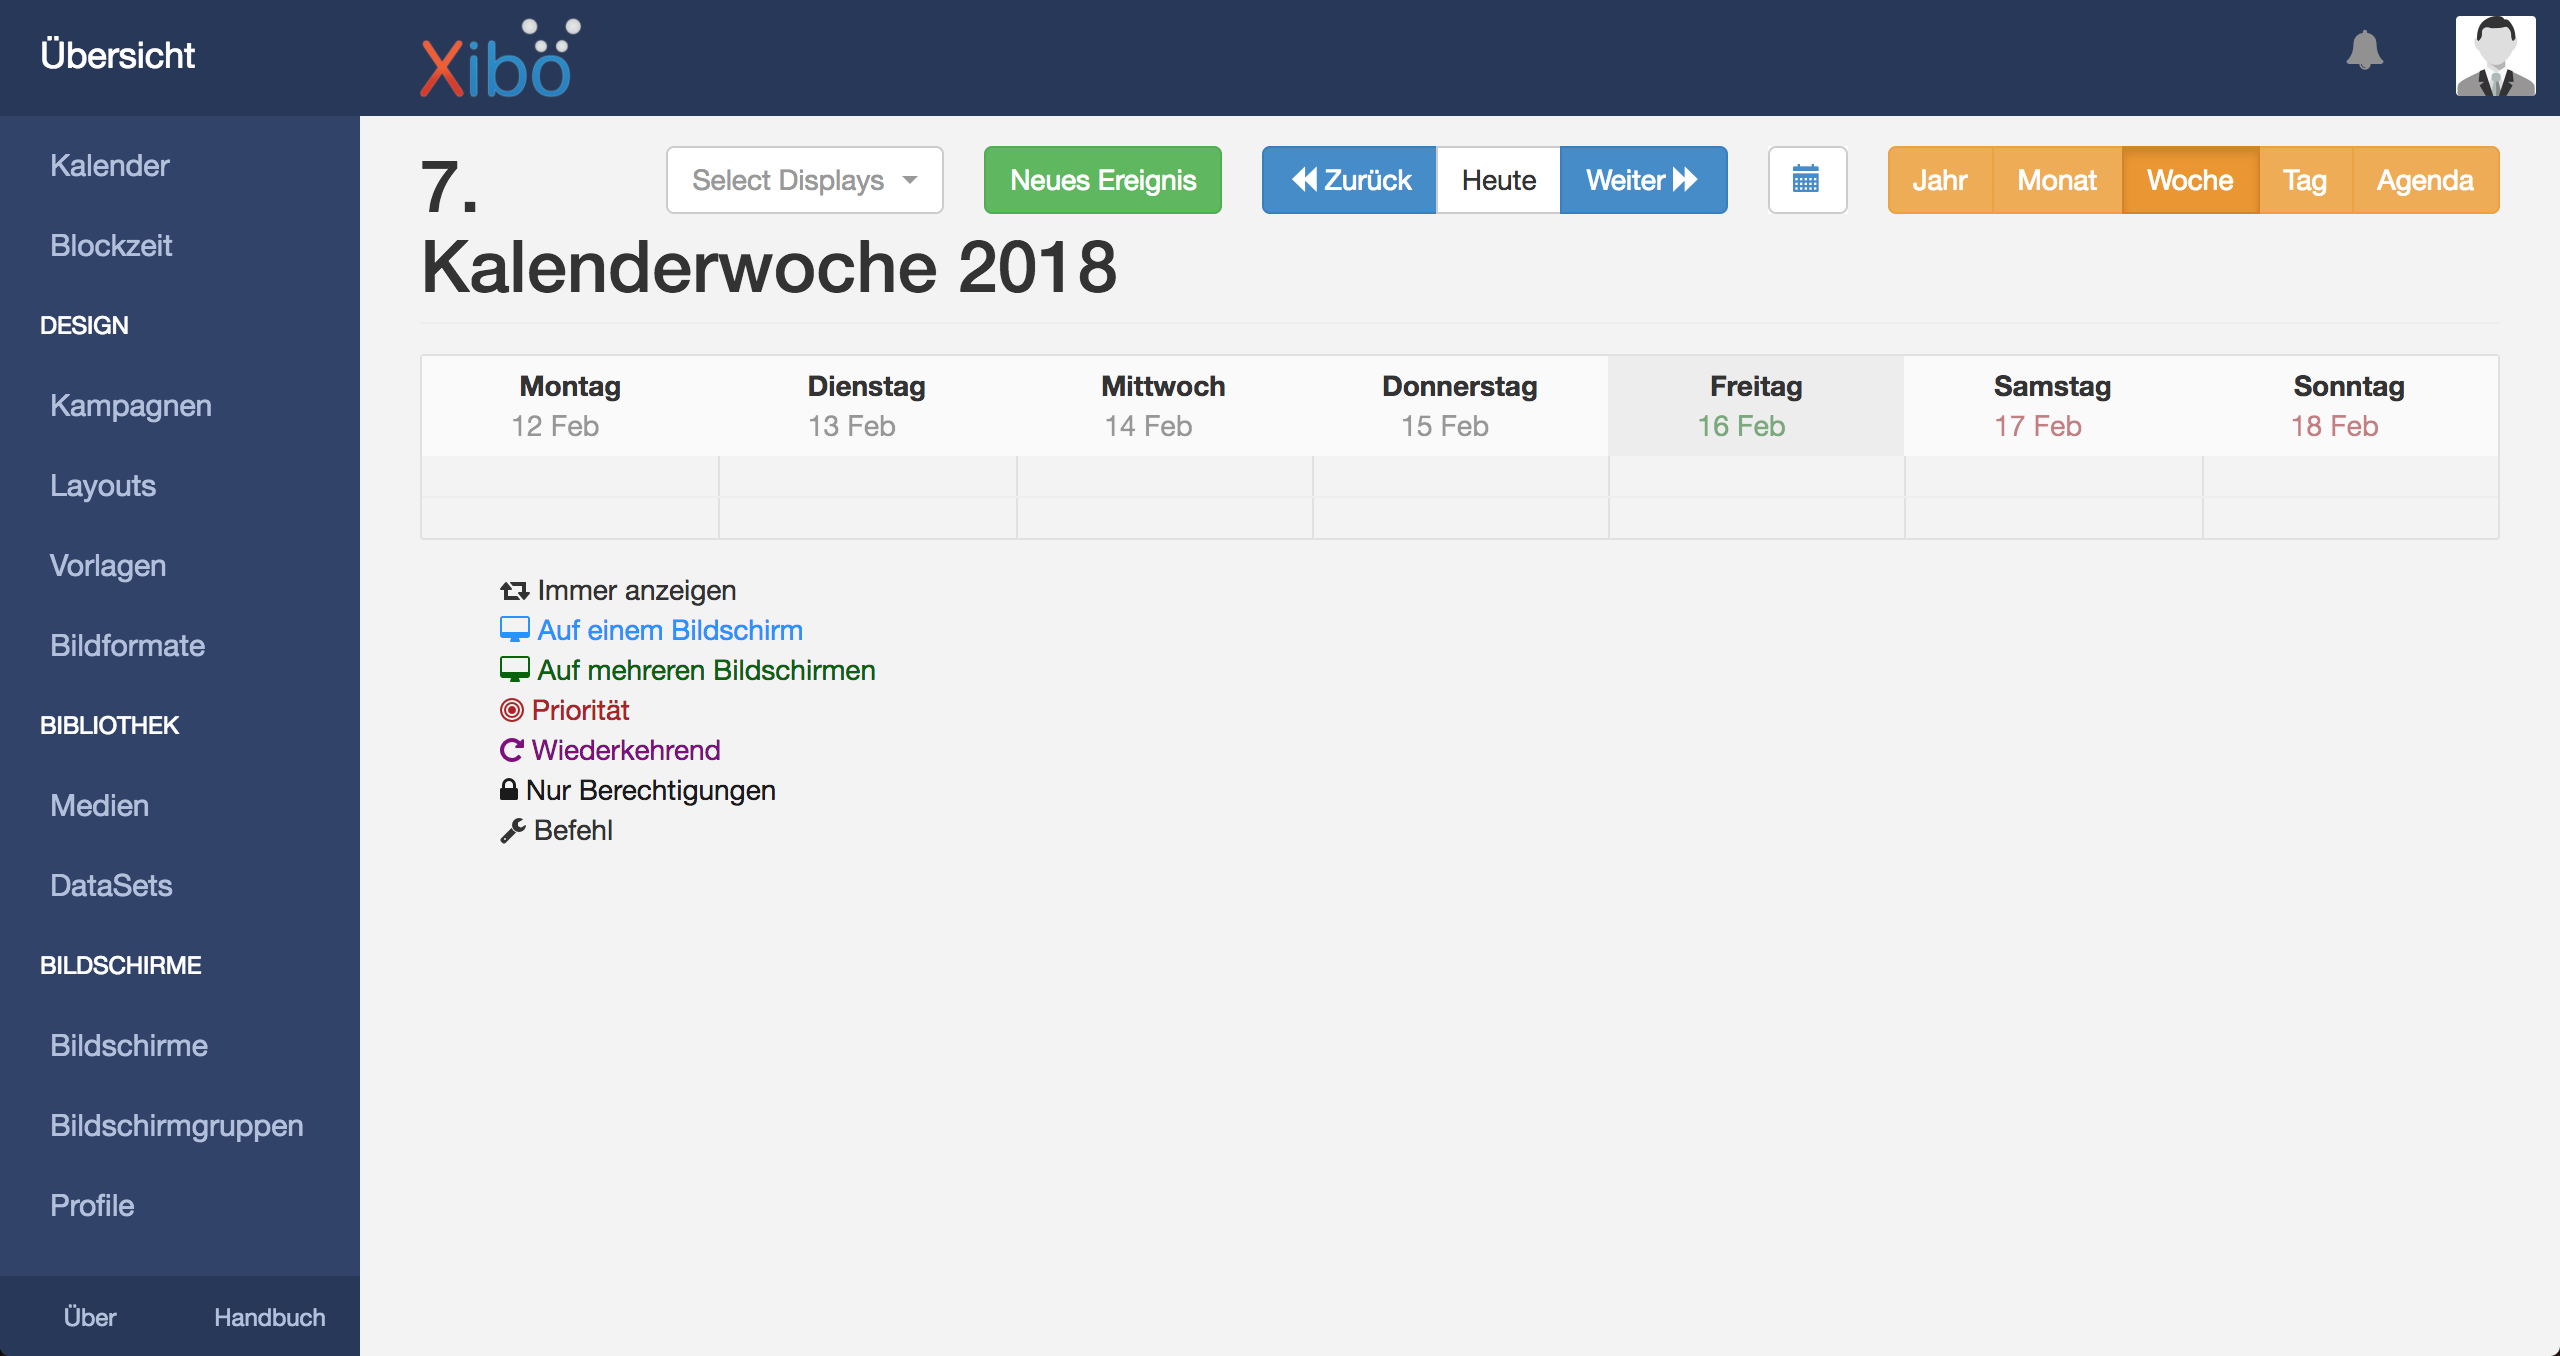
\includegraphics[width=1\textwidth]{images/xibo-basics-calendar}
	\label{img:calendar}
	\caption{XBIO - Kalender}
\end{figure}	
	
	\item {\em Layouts:} 
	Die Layout-Funktion ist einer der wichtigsten Komponenten des Signage Systems. Es beschäftigt sich mit dem Designen der Inhalte. Auf diese Funktion kommen wir noch einmal zurück.
	
	\item {\em Bibliothek:} 
	Die Bibliothek-Funktion ist zuständig für das Verwalten der Medien. Hier können Sie verschiedene Dateien hochladen.  Diese Medien können dann in Layouts eingebunden und angezeigt werden.
	
	\item {\em Benutzer:} 
	Im Menüpunkt Benutzer können neue Benutzer angelegt und bereits bestehende bearbeitet oder gelöscht werden. Dabei gibt es auch ein Rechte-System. Es können auch Datenmengenbegrenzungen pro Benutzer eingestellt werden.
	
	\item {\em Einstellungen:} 
	Der Menüpunkt Einstellungen gibt dem Nutzer die Möglichkeit, verschiedene Optionen zu wählen. So sind zum Beispiel die richtige Zeitzone, E-Mail Benachrichtigungen, wichtige Einstellungen, die für ein einwandfreies Funktionieren des Xibo-Servers zuständig sind einzustellen. Aus den Einstellungen ist auch der CMS geheimer Schlüssel zu finden, der für die Authentifizierung der API Zugriffe zuständig ist herauszulesen.
\end{enumerate}

\section{Designen mit XIBO}\label{sec:designexibo}
Beim Designen von einem neuen Layout im XIBO, muss zuerst die Bildschirmauflösung ausgewählt und dem Layout ein passender Name zugewiesen werden, sowie optional auch eine Beschreibung. 

\textbf{Layout Maske}

\begin{figure}[H]
	\centering
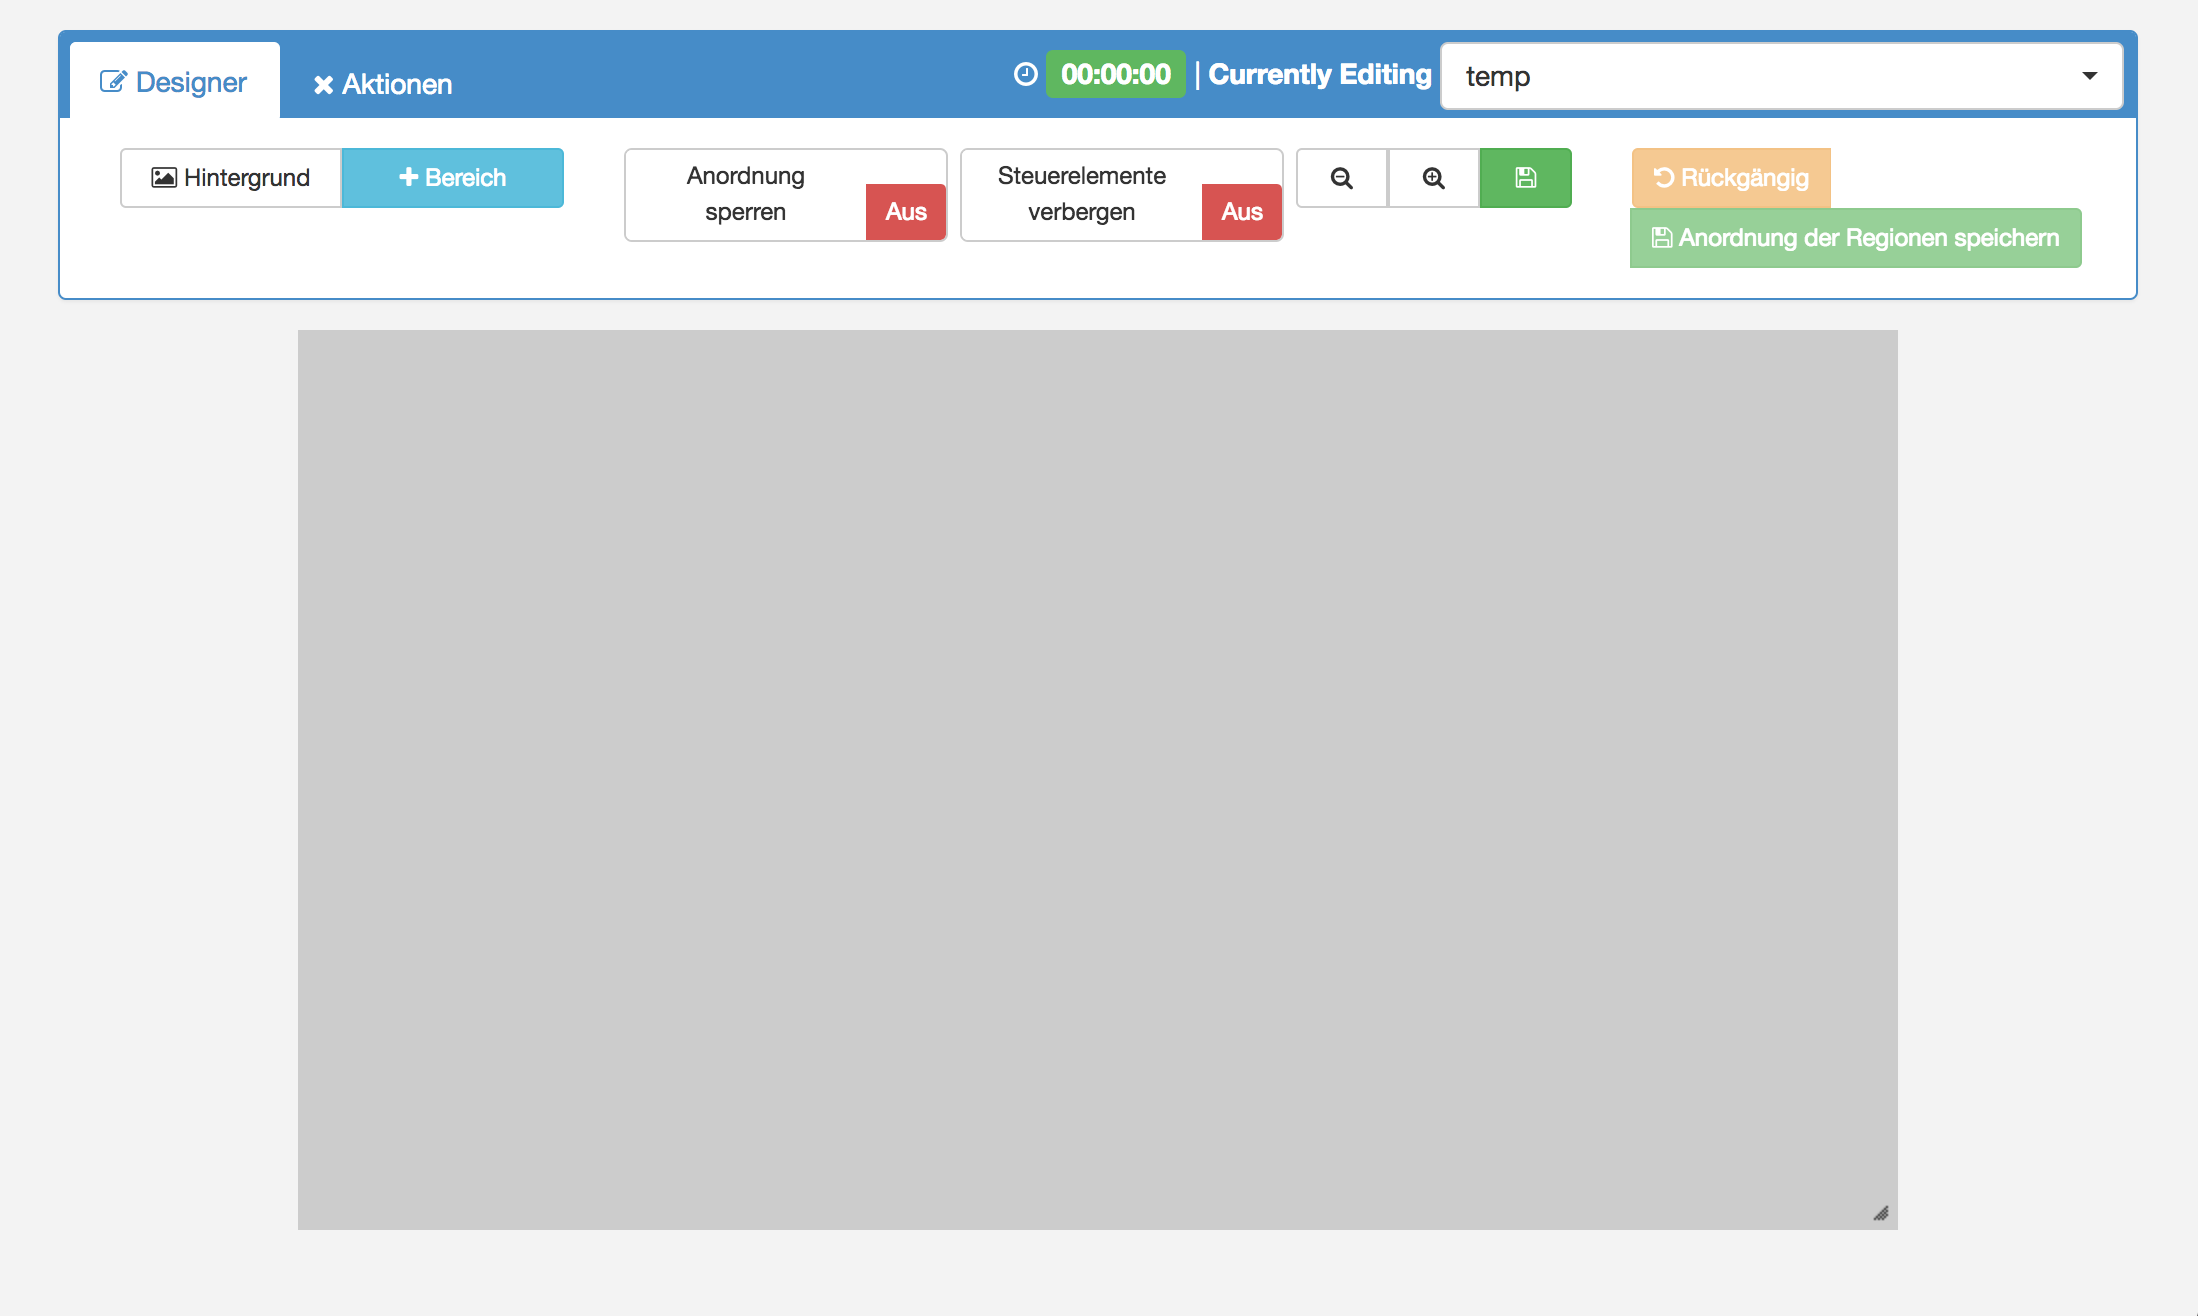
\includegraphics[width=1\textwidth]{images/xibo-basics-designer}
	\label{img:designeLayout}
	\caption{XIBO-Layout designen}
\end{figure}	

Dem Layout kann nun eine Region oder auch mehrere  hinzugefügt werden. Eine Region kann mehrere Widgets enthalten. Mit einem Doppelklick auf die Region kann ein Widget hinzugefügt werden. Es gibt viele verschiedene Arten von Widgets:

\begin{widgettypes}
	\item {\em Bibliothek:} Mit diesem Widget können Elemente aus der Medienbibliothek in der Region angezeigt werden. Dabei werden PowerPoint Formate, Video, Bilder und andere Medien Datentypen unterstützt.
	
	\item {\em Uhr:} 
	Dieser Widgettyp bindet eine Uhr in die Region ein. Es kann entweder eine Uhr im analogen oder digitalen Stil ausgewählt werden.
	
	\item {\em DataSet:} 
	Das DataSet Widget ist sehr wichtig und zeigt einfach gesagt nacheinander Daten aus einem Array, mit Key Value Paaren, an.
	
	\item {\em Wheather:} 
	Das Wheather Widget, in Deutsch Wetter, zeigt das aktuelle Wetter an. Es kann eingestellt werden ob es anhand von den GPS-Daten des Bildschirmes die Wetterdaten anzeigen soll oder ein vorher definierter Ort für die Daten verwendet werden soll.
	
	\item {\em Flash:} 
	Mit dem Flash Widget können Flash Inhalte abgespielt werden.
	
	\item {\em HLS:} 
	Mit dem HLS Widget können HLS Video Streams angezeigt werden.
	
	\item {\em Image:} 
	Mit dem Image Widget können Bilder entweder aus der XIBO Bibliothek angezeigt oder neue hochgeladen werden.
	
	\item {\em Local Video:} 
	Mit dem Local Video Widget können Videos oder Streams angezeigt werden.
	
	\item {\em PDF:} 
	Mit dem PDF Widget können PDFs entweder aus der XIBO Bibliothek angezeigt oder neue hochgeladen werden.
	
	\item {\em PowerPoint:} 
	Mit dem PowerPoint Widget können PowerPoint Präsentationen entweder aus der XIBO Bibliothek angezeigt oder neue hochgeladen werden.

	\item {\em Text:} 
	Mit dem Text Widget können Texte angezeigt werden.
	
	\item {\em Ticker:} 
	Mit dem Ticker Widget können Texte animiert angezeigt werden. Dabei können diese Texte aus einem DataSet oder einem RSS Feed stammen.
	
	\item {\em Webpage:} 
	Mit dem Webpage Widget können Webseiten angezeigt werden.
\end{widgettypes}

Nachdem eines der Widgets erstellt wurde kann das Ergebnis des Layouts mit einer Layout Vorschau kurz überprüft werden.
